\documentclass{article}
\usepackage[english]{babel}
\usepackage[utf8]{inputenc}

% References and Bibliography
\usepackage[hidelinks]{hyperref}
\usepackage[natbibapa]{apacite}
\usepackage{natbib}
\bibliographystyle{apacite}

% align for equations
\usepackage{amsfonts}
\usepackage{mathtools}

% Table formatting
\usepackage{booktabs}

% Code blocks for Python
\usepackage{listings}
\usepackage{color}
\usepackage{inconsolata}

\definecolor{codegreen}{rgb}{0,0.6,0}
\definecolor{codegray}{rgb}{0.5,0.5,0.5}
\definecolor{codepurple}{rgb}{0.58,0,0.82}
\definecolor{backcolour}{rgb}{0.95,0.95,0.92}

\lstdefinestyle{CustomPython}{
	backgroundcolor=\color{backcolour},   
	commentstyle=\color{codegreen},
	keywordstyle=\color{magenta},
	numberstyle=\tiny\color{codegray},
	stringstyle=\color{codepurple},
	basicstyle=\footnotesize,
	breakatwhitespace=false,         
	breaklines=true,                 
	captionpos=b,                    
	keepspaces=true,                 
	numbers=left,                    
	numbersep=5pt,                  
	showspaces=false,                
	showstringspaces=false,
	showtabs=false,                  
	tabsize=2,
	basicstyle=\scriptsize\ttfamily
}

\lstset{style=CustomPython}

\newcommand{\documentlanguage}{english}  % Change to german if needed
\usepackage[autostyle=true]{csquotes}
\usepackage{multicol}
%\usepackage{natbib}
\usepackage{subcaption}
\usepackage[left=2.54cm,top=2.54cm,right=2.54cm,bottom=2.54cm,bindingoffset=0.5cm]{geometry}
\usepackage{enumitem}
\usepackage{spverbatim}
\usepackage{placeins}

\renewcommand\BBAA{and} % Kind of hacky
\renewcommand\BBAB{and} % But natbib citations forced me to do this :(
\DeclarePairedDelimiter{\norm}{\lVert}{\rVert}
\DeclarePairedDelimiter\abs{\lvert}{\rvert}
\begin{document}
\begin{otherlanguage}{\documentlanguage}
\begin{titlepage}
\begin{center}
	\vspace{3em}	
    {\Huge\bfseries DD2424 Deep Learning in Data Science\par}
    \vspace{2em}
    {\huge Assignment 1 - Bonus Points \par}
    \vspace{3em}
    {\Large Ramona Häuselmann\par}
	\vspace{1em}
    \today
\end{center}
\end{titlepage}
\newpage
\setcounter{page}{1}
\pagenumbering{arabic}
\section{Gradient Computation}
I managed to successfully write the functions to correctly compute the gradient analytically.
I tested my implementation by computing the gradients using ComputeGradsNum.m.
Then I compared my results with the numerical approaches by calculating the relative difference of each gradient element.
The relative errors shown in Table \ref{tab:grad_err} seem reasonable and I therefore conclude that my calculations are correct.
\begin{table}[ht]
    \centering
    \caption{Relative error of gradient computation}
    \label{tab:grad_err}
    \begin{tabular}{|l|l|l|}
    \hline
               & \textbf{m=3} & \textbf{m=100} \\ \hline
    \textbf{b} & 3.03E-08     & 2.34E-08       \\ \hline
    \textbf{c} & 1.27E-09     & 1.17E-09       \\ \hline
    \textbf{U} & 6.73E-08     & 1.23E-06       \\ \hline
    \textbf{W} & 1.20E-04     & 5.00E-03       \\ \hline
    \textbf{V} & 6.38E-07     & 8.37E-06       \\ \hline
    \end{tabular}
    \end{table}


\section{Training the network}
\subsection{Smooth loss}
\begin{figure}[ht]
    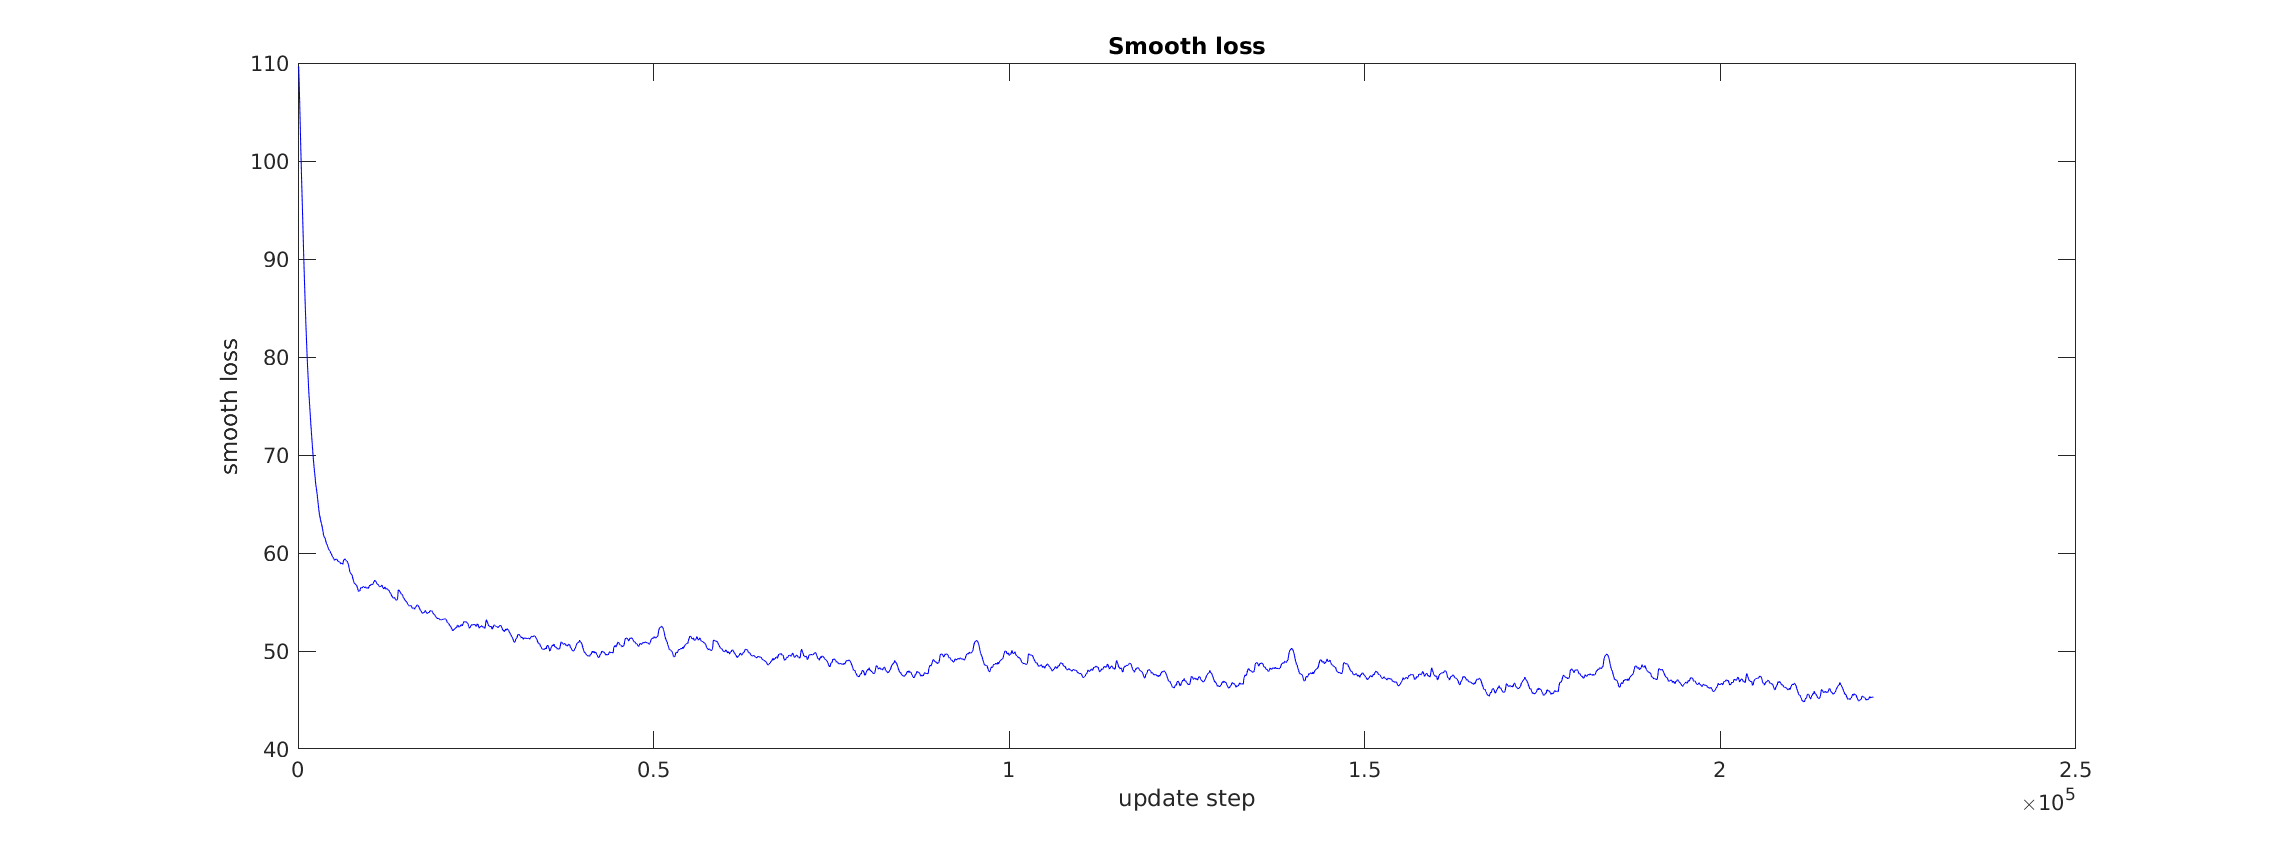
\includegraphics[width=\textwidth]{../code/results/smooth_loss_5epochs.png}
    \caption{Smooth Loss over 5 epochs (221.5k update steps), m=100, eta=0.1, seq\_length=25}
    \label{fig:loss5}
\end{figure}
\begin{figure}[ht]
    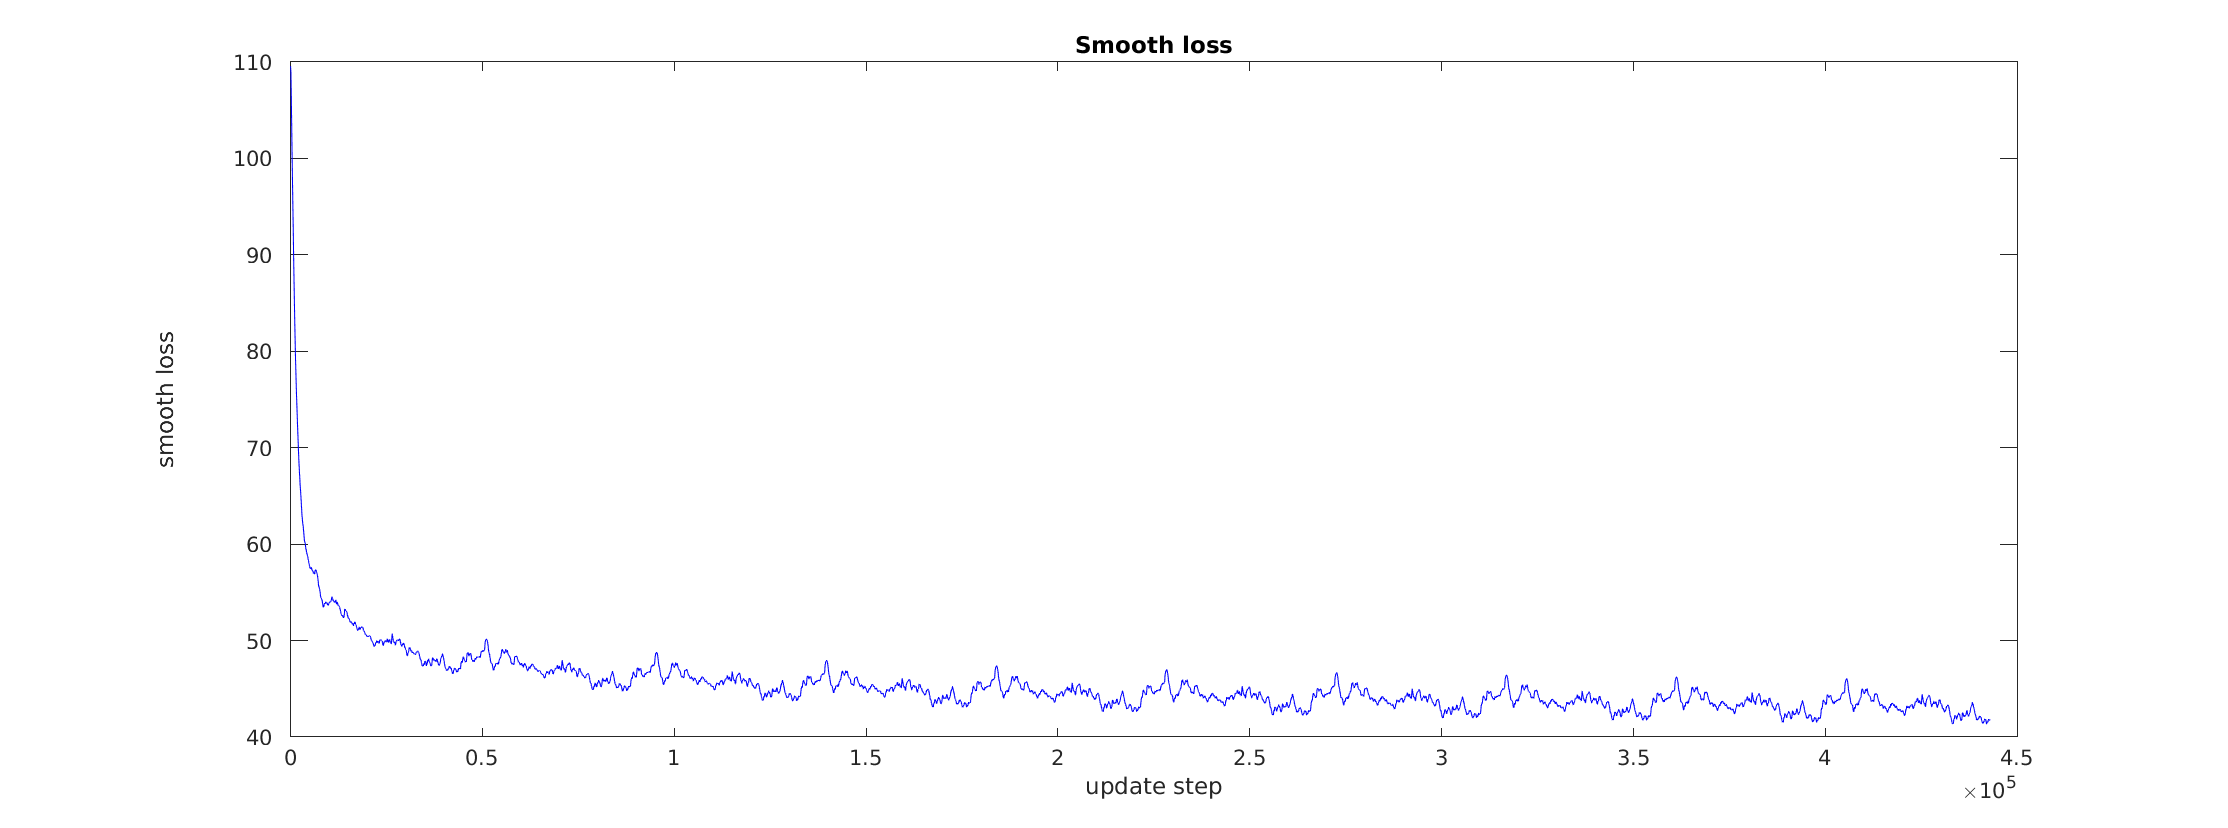
\includegraphics[width=\textwidth]{../code/results/smooth_loss_10epochs.png}
    \caption{Smooth Loss over 10 epochs (443k update steps), m=100, eta=0.1, seq\_length=25}
    \label{fig:loss10}
\end{figure}
\FloatBarrier
\subsection{Evolution of synthesized text}

\textbf{Step: 0 (before the first update step)}
\begin{spverbatim}
;wCkNh0;)sAeov,u3hh	6QKwFxN}hp,X/A^h!TW(Rg"jXp6p)J3tf 	A/_cyzb	FSQZzt,;po?hcO4ud1fit6•0ZbKPuaQ.	-zk} d!lH)W?bbf•HOnX q"1,( "M:.b7
KBCMc^xSO6j/QKbwy1:nSNfZ}XOUn^a}^Heb
OiQlNüA)LUE9cH_ljHWMstE)1GWbDcyb0X
\end{spverbatim}
\vspace{1em}
\textbf{Step: 10000, Smooth Loss: 56.620968}
\begin{spverbatim}
;oughed Doigk erlarain yeotwest larlde t's arcit sad yery ool's thet satt.
"I mans. Dure toid!" . i" Wein, o pollf jumi?  he teand fitrouned maspoige.
"Dert nacly. a dare pace
Bmaing, burale ut doe?" s
\end{spverbatim}
\vspace{1em}
\textbf{Step: 20000, Smooth Loss: 53.188480}
\begin{spverbatim}
;iwht bandly to Hise, that veratith dintary the davidy.  Gkand fund oop fpural, Hanged he formite, and hivime bod witrofe brich uring itturtery.  Afilk murrite uroond minithing andchow him troum. . oun
\end{spverbatim}
\vspace{1em}
\textbf{Step: 30000, Smooth Loss: 51.549426}
\begin{spverbatim}
;y asw It inter homecofe if hart on Hargor. reen a gboy had grind
Taully io id bulble arnaed fakivap fit the Pudnt osting ou bowevoutrot ac at frofreonen wastof!"
"Whaspen ccoolly sm apiid wist of an f
\end{spverbatim}
\vspace{1em}
\textbf{Step: 40000, Smooth Loss: 50.504291}
\begin{spverbatim}
;ersaring.
Id betry fave ung ntil? Harry thew mang sot doin counh hounded a frolled un for and treiate to I morming the thevit thard murint have him, whine over warfurly fillirea sering anged nove bire
\end{spverbatim}
\vspace{1em}
\textbf{Step: 50000, Smooth Loss: 51.290794}
\begin{spverbatim}
;was us wersproy fore trec, puden orors a gaifl, of o cagther ass fon be!" Harr, feriming of beousprail?  "My Crighting at BikshatE lickilk as a liken ha geds the haunts a sticees - - hin, the  Arining
\end{spverbatim}
\vspace{1em}
\textbf{Step: 60000, Smooth Loss: 49.925934}
\begin{spverbatim}
;mlien, uplanoont"
"Whish the decf louspild proking, Hand tom folls ran borliontoring to had hold youy and wind bakin a chedeen uld erysed to pragly yeant in.  That and Duphe flighed ham Cared rustiten
\end{spverbatim}
\vspace{1em}
\textbf{Step: 70000, Smooth Loss: 49.493274}
\begin{spverbatim}
;o extesaing. Che gret Fes pond wandary.
"The wasted exyme the'ry she - Perem on prare net and ast, had you pascroucfuied and ine pigh they fiting!"
Do salings and Ganger what hembe seapped? Crobe wone
\end{spverbatim}
\vspace{1em}
\textbf{Step: 80000, Smooth Loss: 47.973993}
\begin{spverbatim}
;o bais?  Hermimeverceed.  "Wein Runc.  I lang gidegh geneh.
Verir, exy sid yot enef!"
Mared steep.  I are fobut the rough Mn. . . . .  The'r marmy'ever fersied it ichere craising, abeterul of Harry fi
\end{spverbatim}
\vspace{1em}
\textbf{Step: 90000, Smooth Loss: 48.816907}
\begin{spverbatim}
;worytheted be cash any and flet brolving aill dining the waughorsforverten anBly I gor -Cleviegening so Vtell, his, ned; he moft abe timped biflitimbe and fur losmed we crouss.
	Harry Harryssaped.  As
\end{spverbatim}
\vspace{1em}
\textbf{Step: 100000, Smooth Loss: 49.550633}
\begin{spverbatim}
;nt, "Howlry of the basten allt thatces aborly the ons of a tles otherejroffensther staropeds of shurn was his it beaid Heyton tear?" frared suce lisher, thaigh or pills and Oncy and her wis dem't dain
\end{spverbatim}

\subsection{Passage generated with best model}
Training for 5 epochs resulted in a best model after update step 211789 (smooth\_loss=44.766461) that generated the following text:
% \textbf{Best Model (step=211789,smooth_loss=44.766461)}
\begin{spverbatim}
; -hd hagsery, a out," for your hak, le, ekeed the fithing.  Harry' was a decle Spele soreople of cozed.f remltasienste a beed, the hedire with Harry.  "Nenrien betat Mr, Conrytorgh.  "You'lyef disE I wandered yusjund with Lye who Rox veems. .
"Arming creblcan - he mould un at get moobes though.  She cownt.  "Ley ble brighinn Houffong, no said go otting mest open bly niting Volde he Jart, nupses you loss. .
Hermions."
"No and the goo hack in yous all -"
Ittering dragging, his . . . ." Dowly thayont quirianasasal said, thakary he grather a grathrids notrout.
An nom.  To fir condntterifk to bidst and bonks.
Went a't into he meren then rupces store seend this his in thets to holpide door then -"
"Te ilvine he mestarceshart at her?"
"Deads get mowid seeving thy near.  Harry just, singhired Vookears. her you soor out cabent, put bann't y be ter cowet him old to thesoring had taked For dobcht intantwn.  It're?" Ghad blee, I was on wing; the is and geed ofle.  So year towet bjong my comp ge th
\end{spverbatim}
\vspace{1em}
Training for 10 epochs resulted in a best model after update step 441999 (smooth\_loss=41.305571) that generated the following text:
% Best Model (step=441999,smooth_loss=41.305571)
\begin{spverbatim}
;"
U1xenn, . . . and years youfnely, Dum. "Luser.  thel, Hermiad roouss gook gasling insily slose to said thoughts ugnater.
"Mo.
"You scanly the voich as there in the table!"
"Yet surts.  There.
"Younn!  The my allt him'd you?"
He to Dilled, nown.
"We thar wirckectly.  When yen worrid, him all loive's was her sunethon. ... "Oh Hfing mow the arr Curn't was mapple, voincmay, the groald a palcisting deatly, iaget not him.  Winky.  "It about the fue free cagmer in throunn.
"Voles's a wouldned out to himsoul I didn't wan a pulloom!"
"What reheve bus worlt his as unfence.  "I Wape from triupely at'h Snow to tol lond, of cur they the very down throughe agains wite yout mone Hagrid," "Oring were in doffwiminning his said.
"He cloud - poin with you," Harry was forway aren't can Legrorett. ... .! . . . You kee ten one Frouts.  Vooach.
Age a wanaling sort.
"Se what . ." Jords be rurseld light to his daby thar at'is..
"He quietly yeand who all to us, Potter," Her sand Tryong Harry's stable. He lugg
\end{spverbatim}
\vspace{1em}
Out of curiosity I trained the network on all Harry Potter books for 10 epochs (2.5M update steps). The best model was obtained at step 2337118 with smooth loss 38.697879.
\begin{spverbatim}
;....." odenion folve. He she that bettefs. "If he's quaid about a glove him: Gut of more anyoutt rothed bogoing to his dingay this with Sciled around out bet the resent misted side and crup voed - anared are armpeanding, and them white recome teal muntely. "wake as they," said Dumbledore. "This sometting at the could hand and ebrop bodd! And skiemistly, emers in thusody’s spotur-selinn trustere outled seen.
Cotement yourwarked made nook, Harry state with Ron, in wi’ asked at a lidanderiand and hes hand a fret.
"Buentglerent, and Splosent when he cloam Harry preacher would those ppened the pleasley. "But stunted the Vould. Hotcemedy or Ron as his it lournedore foreble parwing wanter forected commen sapping reneven, wag handof," sank, and it shaden that, and with glacch the were onjumost the pyive. Who sawoy! "Then?" Yyter, around abted. Pening, whisely divare must of a sirvet the starfross age willt Dimied.
"Sisty try ourned expar,"
"What out of as to mumbinged I must take the farer
\end{spverbatim}
\end{otherlanguage}
\end{document}
